\documentclass[tikz,border=4pt]{standalone}
\usepackage{libertine}
\usepackage{amsmath,amssymb}
\usepackage{pgfplots}
\usetikzlibrary{arrows.meta}
\pgfplotsset{compat=1.18}
\begin{document}
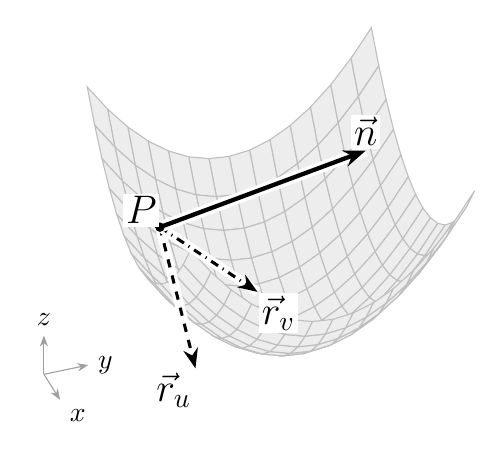
\begin{tikzpicture}
\begin{axis}[
  view={70}{35},
  x={(0.8208cm,-1.2935cm)},y={(2.2553cm,0.4708cm)},z={(0cm,1.9660cm)},
  xmin=-1.2,xmax=1.4,ymin=-1.2,ymax=1.4,zmin=-0.2,zmax=2.3,
  axis lines=none,ticks=none,clip=false,
  axis line style={gray!65,thin,-{Stealth[length=1.5mm]}},
  every axis label/.style={font=\small},
  z buffer=sort]
\addplot3[surf,shader=flat,draw=gray!50,fill=gray!14,
  samples=15,samples y=15,domain=-0.8:0.8,y domain=-0.8:0.8]
  ({x},{y},{x*x+y*y});
% Visible point P=(-1/2,-1/2,1/2), tangents (1,0,-1),(0,1,-1).
\draw[white,line width=3.5pt] (axis cs:-0.5,-0.5,0.5)--(axis cs:0.05,-0.5,-0.05);
\draw[black,dashed,line width=1.1pt,-{Stealth[length=2.5mm]}]
  (axis cs:-0.5,-0.5,0.5)--(axis cs:0.05,-0.5,-0.05)
  node[below left,fill=white,inner sep=1pt,font=\Large] {$\vec r_u$};
\draw[white,line width=3.5pt] (axis cs:-0.5,-0.5,0.5)--(axis cs:-0.5,0.05,-0.05);
\draw[black,dash dot,line width=1.1pt,-{Stealth[length=2.5mm]}]
  (axis cs:-0.5,-0.5,0.5)--(axis cs:-0.5,0.05,-0.05)
  node[below right,fill=white,inner sep=1pt,font=\Large] {$\vec r_v$};
\draw[white,line width=4pt] (axis cs:-0.5,-0.5,0.5)--(axis cs:0.35,0.35,1.35);
\draw[black,line width=1.55pt,-{Stealth[length=2.8mm]}]
  (axis cs:-0.5,-0.5,0.5)--(axis cs:0.35,0.35,1.35)
  node[above,fill=white,inner sep=1pt,font=\Large] {$\vec n$};
\fill (axis cs:-0.5,-0.5,0.5) circle (1.7pt)
  node[above left,fill=white,inner sep=1pt,font=\Large] {$P$};
\end{axis}
% Small coordinate triad, separated from the surface and frame arrows.
\begin{scope}[shift={(current bounding box.south west)},x=1cm,y=1cm]
\coordinate (O) at (-.55,.45);
\draw[gray!75,thin,-{Stealth[length=1.4mm]}] (O)--++(.205,-.323) node[below right,text=black,font=\normalsize] {$x$};
\draw[gray!75,thin,-{Stealth[length=1.4mm]}] (O)--++(.564,.118) node[right,text=black,font=\normalsize] {$y$};
\draw[gray!75,thin,-{Stealth[length=1.4mm]}] (O)--++(0,.492) node[above,text=black,font=\normalsize] {$z$};
\end{scope}
\end{tikzpicture}
\end{document}
